%% ---------------------------------------------------------------------------
%%  IEEEtran journal article.  Build:  tectonic article.tex
%%  or:  pdflatex article && pdflatex article
%%  Figures are generated from ../results by make_figures.py.
%% ---------------------------------------------------------------------------
\documentclass[journal]{IEEEtran}
\usepackage{cite}
\usepackage{amsmath,amssymb}
\usepackage{graphicx}
\usepackage{booktabs}
\usepackage{textcomp}
\usepackage{url}
\renewcommand{\topfraction}{0.92}
\renewcommand{\bottomfraction}{0.85}
\renewcommand{\textfraction}{0.06}
\renewcommand{\floatpagefraction}{0.75}
\newcommand{\X}{\texttt{x}}

\begin{document}

\title{X-Freedom Is Not Validity: Certification-Gated Gate-Level Switching
Activity for Pre-Silicon Power Analysis}

\author{Maulik~Timbadiya,~\IEEEmembership{Independent Researcher}}

\markboth{Certification-gated gate-level switching activity}{Timbadiya}

\maketitle

\begin{abstract}
Gate-level simulation (GLS) is the preferred source of switching activity for
pre-silicon power analysis, but most flip-flops in a typical design have no
reset and power up unknown (\X). Unknown values propagate pessimistically
through gates and optimistically through behavioural RTL, so the two models can
execute different instruction streams. The common mitigation, simulator register
initialization, removes every \X{} but initializes each model independently. On
a synthesized 32-bit pipelined processor with 680 sequential elements, 95.0\% of
them non-resettable, independent randomization reproduced the RTL execution in
0 of 20 seeds while leaving no unknown values, under-reported average signal
power by 88.6\%, and displaced the peak-power cycle from 70 to 0. We study a
method that treats gate-level activity as inadmissible until correspondence is
demonstrated: one power-up state vector is applied to the non-resettable state of
both models through a synthesis-derived correspondence map, both models run
concurrently, every mapped element is compared each cycle with a four-state
comparison, and activity is released only for the certified cycle window.
Co-initialization reproduced the RTL execution in 20 of 20 seeds. We report the
\X-contamination front, the dependence of peak-power timing on legal power-up
state, a checkpoint-transplant variant, the blind spots of two-state comparison,
and the method's cost, which was below run-to-run timing noise at this design
size. Equivalence results reproduce bit-identically on three independently
implemented simulators, and every result regenerates from a licence-free
harness.
\end{abstract}

\begin{IEEEkeywords}
Gate-level simulation, X-propagation, power estimation, switching activity,
pre-silicon verification, equivalence, electronic design automation.
\end{IEEEkeywords}

\section{Introduction}

\IEEEPARstart{P}{ower} is a first-order design constraint, and power estimates
are needed long before silicon exists. Switching activity recorded from
gate-level simulation is attractive for this purpose because it needs no
inference: every net that will exist in silicon exists in the netlist, including
clock-gating structure and synthesized logic. Activity is recorded as VCD, FSDB
or SAIF and consumed by a power analysis engine.

The obstacle is the unknown value. Reset inputs cost area, load the reset
distribution network and consume power, so designers add them only where control
logic requires a known state. Register files, memories, queues, configuration
registers and pipeline datapaths are commonly non-resettable. In the processor
studied here, 646 of 680 sequential elements have no reset.

Those elements hold \X{} when simulation starts. In gates, \X{} propagates
\emph{pessimistically}: a cell with an unknown input usually produces an unknown
output even where silicon would settle to a known value. In behavioural RTL,
\X{} is handled \emph{optimistically}: an \texttt{if} whose condition is unknown
takes its \texttt{else} branch and a \texttt{case} with an unknown selector
executes its \texttt{default}~\cite{ieee1364,ieee1800}. The two models are
logically equivalent as functions yet, from an unknown start, need not execute
the same program.

The usual remedy is a simulator option that assigns known values to storage at
time zero. It removes every visible \X. This article shows that removing \X{} is
not the same as making activity valid, and studies a method that makes validity
something that is checked rather than assumed.

\subsection{Contributions}
\begin{enumerate}
\item We measure that independent initialization of the netlist removes all
      unknown values yet reproduced the RTL execution in 0 of 20 seeds, with
      signal-power error of $-88.6\%$ and a displaced peak-power cycle.
\item We describe \emph{certification-gated release}: gate-level activity is
      admitted to power analysis only for a cycle window over which all mapped
      state of a co-initialized gate-level model and RTL model was identical.
      We document practical hazards: synthesis renaming, reset-edge overwrites,
      and optimizer removal of referenced flops.
\item We report the \X-contamination front, a latent dependence on power-up
      state exposed by the method, the sensitivity of peak-power timing to legal
      power-up state, a checkpoint-transplant variant, and a measurement of what
      a two-state comparison cannot see.
\item We confirm the equivalence results on three independently implemented
      simulators and release a harness that regenerates every table and figure
      using only open-source tools.
\end{enumerate}

\section{Background}

\subsection{Gate-level activity for power}
A power engine combines per-net switching activity with cell and wire models.
Activity recorded at RTL must be propagated through an inferred structure to
estimate nets absent from the RTL; activity recorded at gate level needs no such
step. The price is that the gate-level run must actually execute the intended
workload.

\subsection{Four-valued semantics}
Verilog and SystemVerilog model each bit as 0, 1, \X{} or \texttt{z}. Consider a
branch in a pipelined processor:
\begin{center}\small
\texttt{if (taken) pc <= target; else pc <= pc + 1;}
\end{center}
If \texttt{taken} is \X, RTL simulation takes the \texttt{else} branch and the
program counter stays known. In the synthesized netlist the same decision is a
multiplexer whose select is \X, so the program counter becomes \X. An array write
through an unknown index is similar: RTL writes nothing, while the gate-level
address decoder drives unknown enables into many elements.

\subsection{Existing mitigations}
Commercial simulators provide register-initialization options (for example the
\texttt{+vcs+initreg} family) that set storage to zero, one or pseudo-random
values at time zero, and X-propagation modes that make RTL semantics more
pessimistic. Initializing netlist storage randomly before reset is also
known~\cite{p8000950}. Work on \emph{false} \X{} computes when a gate's output
is known despite unknown inputs and forces the correct
value~\cite{p9965575,p10726180,p9058452}. Capturing RTL state at some cycle and
mapping it onto gate-level nodes to start a shorter gate-level run is also
known~\cite{p10540462}. Estimating power directly from RTL activity with
gate-level cell models avoids gate-level simulation altogether~\cite{p6598209}.

What these approaches share is that none establishes, cycle by cycle, that the
gate-level model is executing the same workload as the RTL model, and none
conditions the use of harvested activity on that fact.

\section{Method}

Fig.~\ref{fig:flow} summarizes the flow.

\begin{figure}[!t]
\centering
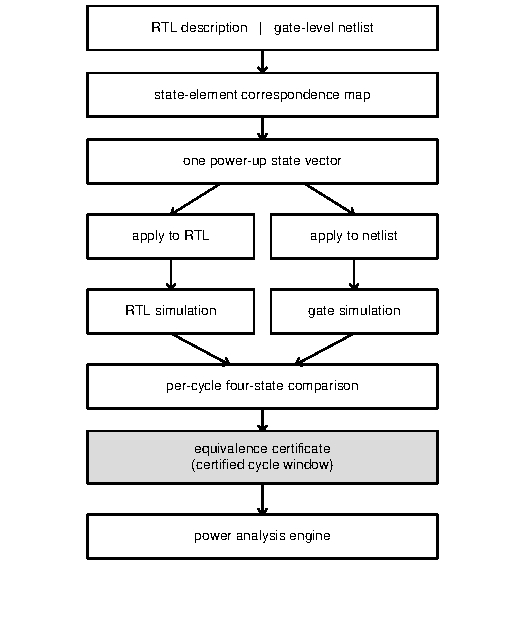
\includegraphics[width=\columnwidth]{figures/fig_flow.pdf}
\caption{Method flow. Activity reaches the power engine only for cycles covered
by an equivalence certificate.}
\label{fig:flow}
\end{figure}

\subsection{State-element correspondence}
Synthesis gives mapped cells synthetic instance names, but the nets they drive
keep design-derived names. A single-stage name match is not enough because
optimization merges nets and promotes port names. We union net-name aliases from
two graphs: one captured after elaboration and before optimization, where RTL
register names and the wires and ports assigned from them coexist, and one
captured from the mapped netlist. Each equivalence class is reduced to a
canonical name, preferring a name declared as a register in the RTL (the only
legal target of a procedural deposit), then the output of an RTL sequential
element, then anything other than a promoted port. In a production flow the
matched state points reported by a formal equivalence checker are a better
source: they survive retiming and report what could not be matched.

\subsection{Provenance binding}
A vector is meaningful only for the netlist it was derived from. The map carries
a SHA-256 digest of the RTL source, the netlist, the cell library and the sorted
map contents; a vector is refused when the digest does not match the models
being simulated. This mechanizes the rule that the comparison reference must be
the RTL revision that produced the netlist.

\subsection{Co-initialization}
One vector assigns a known value to each mapped element and is emitted twice:
once addressing RTL storage and once addressing netlist cell instances. Values of
resettable elements are established by the reset sequence, identically in both
models. What matters is not that the state is known but that it is
\emph{shared}.

\begin{figure}[!t]
\centering
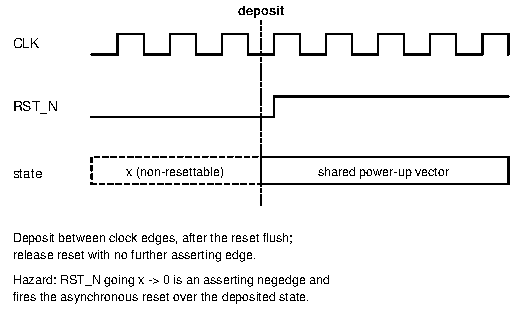
\includegraphics[width=\columnwidth]{figures/fig_reset.pdf}
\caption{Applying the deposit so that reset cannot overwrite it.}
\label{fig:reset}
\end{figure}

Two hazards defeat a naive deposit. First, an asynchronous reset declared
without an initial value makes an \X{}-to-0 transition at time zero; that
transition is an asserting edge and fires the reset path over anything already
deposited (Fig.~\ref{fig:reset}). Second, when deposits use hierarchical
references, the simulator's elaboration optimizer must be told to preserve the
referenced instances; one commercial simulator in our study required explicit
access options before the deposits would bind.

\subsection{Lockstep comparison}
Both models run under identical stimulus. After each active clock edge and a
settling delay, the mapped state of each model is sampled as a packed
concatenation in canonical order and compared with a single four-state case
inequality. Only when that fails is a bitwise scan run. For very large state the
concatenation can be split into chunks so the scan touches one chunk.

The comparison must be four-state. A comparison that first reduces each bit to
two states maps \X{} onto 0, cannot observe unknown values, and misses any
divergence confined to bits whose reference value is 0. Section~\ref{sec:twostate}
quantifies this.

\subsection{Divergence localization and classification}
On failure we report the earliest cycle and earliest diverging element, and
classify it: \emph{X-origin} when the gate-level value is unknown and the RTL
value known; \emph{RTL-unknown} when the reverse holds, which occurs when only the
netlist was initialized; and \emph{value mismatch} when both are known and
differ. The retirement interface of the processor (valid, program counter, opcode,
destination, value) is sampled in the same cycle so that a divergence is reported
against the instruction being retired.

\subsection{Certification-gated release}
When comparison holds over a window, an equivalence certificate records the
window, the number of elements compared, the vector and the provenance digest.
Activity is supplied to the power engine only for certified cycles. Transitions
with an unknown or high-impedance endpoint are counted separately and reported as
a credibility metric.

\subsection{Constrained power-up families}
Some state is guaranteed by boot firmware or reset; the rest is free. Fixing the
guaranteed subset and sweeping the rest defines a family of legal power-up
states, each of which must certify. The distribution of activity and power over
the family is a measurement unavailable from an \X-contaminated run.

\subsection{Checkpoint transplant}
RTL state captured at a chosen cycle can be applied to the netlist through the
same map so that gate-level simulation starts mid-workload. Transferring state
this way is known~\cite{p10540462}; the difference here is that the RTL model
keeps running and the transplanted window is itself certified.

\section{Experimental Methodology}

\subsection{Designs}
\emph{tinycpu} is a three-stage 32-bit pipelined processor with an eight-entry
register file, an eight-entry data memory, write-back forwarding, a branch with
one delay slot and an external 64-word instruction ROM. Its operations are add,
subtract, and, or, xor, shift left and right, load-immediate, load, store,
branch-if-nonzero and halt. Reset reaches the program counter, the halt flag and
the first-stage valid bit (34 flops). The register file, data memory and pipeline
datapath, including the second-stage valid bit, are non-resettable.

\emph{core\_small} is an 8-bit variant with a four-entry register file and a
16-word internal ROM, with 58 sequential elements. It exists so that the whole
experiment fits in two source files that can be run unchanged on any
SystemVerilog simulator.

\subsection{Cell library and synthesis}
The library has eleven combinational cells (inverter, buffer, two-input NAND, NOR,
AND, OR, XOR, XNOR, a two-input multiplexer, AOI21, OAI21), a D flip-flop without
reset and a D flip-flop with asynchronous active-low reset, described in Liberty
and in Verilog models with ordinary four-state behaviour. Synthesis used
Yosys~0.68~\cite{yosys} (process, memory mapping, technology mapping, flop mapping
to the library, and ABC optimization against the library).

\subsection{Workload}
The tinycpu program begins with a boot-style branch on register r5 before any
instruction has written it, then initializes four registers and runs a
twelve-iteration loop of add, xor, shift, store, subtract and increment, followed
by a load, an xor and a halt. The reference execution halts after 107 cycles.
The core\_small program branches in the same way on an unwritten register. A
branch that depends on uninitialized state is the kind of defect gate-level
simulation is expected to expose.

\subsection{Experimental arms}
\emph{Arm A} is RTL simulation without initialization, as simulators do by
default. \emph{Arm B} is gate-level simulation without initialization.
\emph{Arm C} assigns independent pseudo-random values to every netlist flop and
leaves the RTL untouched, emulating a register-initialization option.
\emph{Arm E} applies one vector to both models: the all-zeros vector; 20
pseudo-random vectors; and 20 pseudo-random vectors with r5 fixed to 0. In the
tinycpu harness the vector is applied at time zero and reset then re-establishes
resettable elements; in the core\_small testcase it is applied to non-resettable
elements after the reset flush. The effect is the same.

\subsection{Activity and power model}
Clean 0$\leftrightarrow$1 transitions per net are read from VCD and attributed to
the driving cell. Switching energy per output transition ranges from 0.5\,fJ
(inverter) to 7.0\,fJ (resettable flop). Clock energy is charged at 2.5\,fJ or
2.8\,fJ per flop per edge and leakage at 0.8\,nW per library area unit, with a
10\,ns clock. Clock and leakage contribute 181.3\,\textmu W of the reference's
191.3\,\textmu W, so arms are compared on \emph{signal} power. The energy values
are synthetic; absolute power is illustrative and only relative differences are
meaningful.

\subsection{Tooling}
All experiments ran on Icarus Verilog~13.0~\cite{icarus} and Yosys~0.68 with
Python~3. The core\_small testcase was additionally run on Synopsys VCS
X-2025.06-SP1 and Siemens QuestaSim~2025.2. Timings are wall-clock medians over
21 repetitions on one workstation.

\section{Results}

\subsection{Synthesis and correspondence}

\begin{table}[!t]
\caption{Synthesized designs}
\label{tab:synth}
\centering\footnotesize
\begin{tabular}{lrr}
\toprule
 & tinycpu & core\_small \\
\midrule
Cells                    & 3{,}496 & 336 \\
Sequential elements      & 680 & 58 \\
\quad non-resettable     & 646 (95.0\%) & 52 (89.7\%) \\
\quad resettable         & 34 & 6 \\
Mapped to RTL storage    & 680 of 680 & 58 of 58 \\
Renamed by synthesis     & 121 (17.8\%) & 15 (25.9\%) \\
\bottomrule
\end{tabular}
\end{table}

\begin{table}[!t]
\caption{tinycpu state renamed by synthesis}
\label{tab:rename}
\centering\footnotesize
\begin{tabular}{llr}
\toprule
Netlist name & RTL storage & Bits \\
\midrule
\texttt{retire\_val\_o} & \texttt{alu\_r\_w} & 32 \\
\texttt{retire\_pc\_o}  & \texttt{pc\_w}     & 32 \\
\texttt{pc\_o}          & \texttt{pc}        & 26 \\
\texttt{imm\_d}         & \texttt{ir\_d}     & 16 \\
\texttt{imem\_addr}     & \texttt{pc}        & 6 \\
\texttt{retire\_op\_o}  & \texttt{op\_w}     & 4 \\
\texttt{retire\_rd\_o}  & \texttt{rd\_w}     & 3 \\
\texttt{retire\_v\_o}   & \texttt{v\_w}      & 1 \\
\texttt{halted\_o}      & \texttt{halted}    & 1 \\
\bottomrule
\end{tabular}
\end{table}

Table~\ref{tab:synth} characterizes both designs and Table~\ref{tab:rename} the
renames. Every sequential element resolved to RTL storage, but 17.8\% of tinycpu's
carry a netlist name different from the storage they hold: a register surfaces
only under the port it drives, the program counter is split across two names, and
the instruction register partly appears under a wire that selects a field of it.
A deposit script matching names directly would seed these incorrectly.

\subsection{Uninitialized gate-level simulation}

\begin{figure}[!t]
\centering
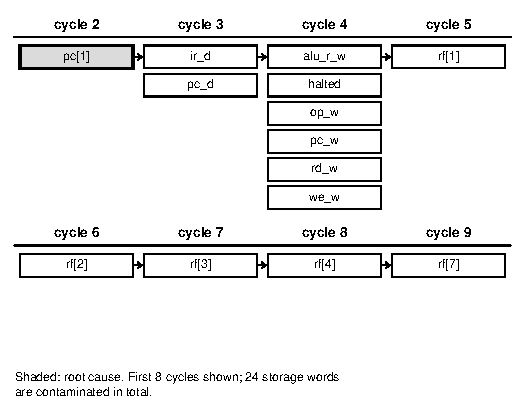
\includegraphics[width=\columnwidth]{figures/fig_cone.pdf}
\caption{Measured \X-contamination front in arm B: the first cycle at which each
storage word diverges from RTL.}
\label{fig:cone}
\end{figure}

Arm B diverges at cycle 2. State comparison places the root at bit 1 of the
program counter: RTL holds 1 and the netlist holds \X{}, an X-origin divergence
attributed to the boot branch retiring at program counter 0. From there the front
spreads through the fetch and decode registers at cycle 3, the execute and
write-back registers at cycle 4, and one register-file entry per cycle afterward
(Fig.~\ref{fig:cone}), reaching 24 storage words. 106 of 107 compared cycles
diverge and the run never halts within a 400-cycle limit. Of all transitions
recorded, 67.3\% have an unknown endpoint.

\subsection{Independent randomization}
Arm C contains no unknown values once simulation starts, and diverges anyway. In
the recorded seed the first diverging element is bit 0 of the execute-stage
result register at cycle 1, an RTL-unknown divergence. The netlist takes the boot
branch that RTL declined and halts after 5 cycles instead of 107. Across 20 seeds
the netlist reproduced the RTL execution 0 times and halted after 5 cycles every
time. A check for unknown values passes in every one of these runs.

\begin{table}[!t]
\caption{Reproduction of the RTL execution (tinycpu). First divergence
is given as cycle and class.}
\label{tab:equiv}
\centering\footnotesize
\begin{tabular}{lccc}
\toprule
Initialization & Repro. & Unknown & First \\
               & RTL    & trans.  & div. \\
\midrule
None (B)          & no    & 67.3\% & 2, X-origin \\
Random (C)        & 0/20  & 0.0\%  & 1, RTL-unk. \\
Zeros (E)         & yes   & 0.0\%  & none \\
20 seeds (E)      & 20/20 & 0.0\%  & none \\
Constrained (E)   & 20/20 & 0.0\%  & none \\
\bottomrule
\end{tabular}
\end{table}

\subsection{Co-initialization}
With the all-zeros vector both models run 107 cycles and all 680 elements agree on
every cycle. All 20 random vectors certify, as do all 20 constrained vectors
(Table~\ref{tab:equiv}).

\subsection{A latent dependence exposed}
The co-initialized runs disagree with each other, not with RTL. Under the zeros
vector both models fall through the boot branch and run 107 cycles; under every
random vector both take the branch and halt after 5. Which program runs depends on
the power-up value of r5. Arm A never shows this, because RTL resolves the
unknown branch condition the same way every time. Making both models start from
the same known state turned a masked defect into an observable one.

\subsection{Activity and power}

\begin{table}[!t]
\caption{Activity and power over a common 107-cycle window}
\label{tab:power}
\centering\footnotesize
\begin{tabular}{lrrrrr}
\toprule
Arm & Toggles & Err. & $P_{sig}$ & Peak & Peak \\
    &         &      & (\textmu W) & (\textmu W) & cycle \\
\midrule
Co-init (ref.) & 71{,}910 & ---        & 10.05 & 188.2 & 70 \\
Indep.\ random & 4{,}502  & $-93.7\%$  & 1.15  & 214.6 & 0 \\
No init        & 757      & $-98.9\%$  & 0.06  & 173.3 & 5 \\
\bottomrule
\end{tabular}
\end{table}

\begin{figure}[!t]
\centering
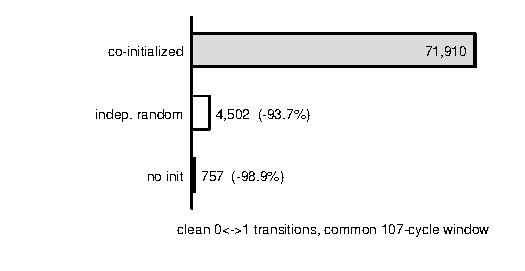
\includegraphics[width=\columnwidth]{figures/fig_activity.pdf}
\caption{Clean transitions recorded in each arm.}
\label{fig:activity}
\end{figure}

\begin{figure*}[!t]
\centering
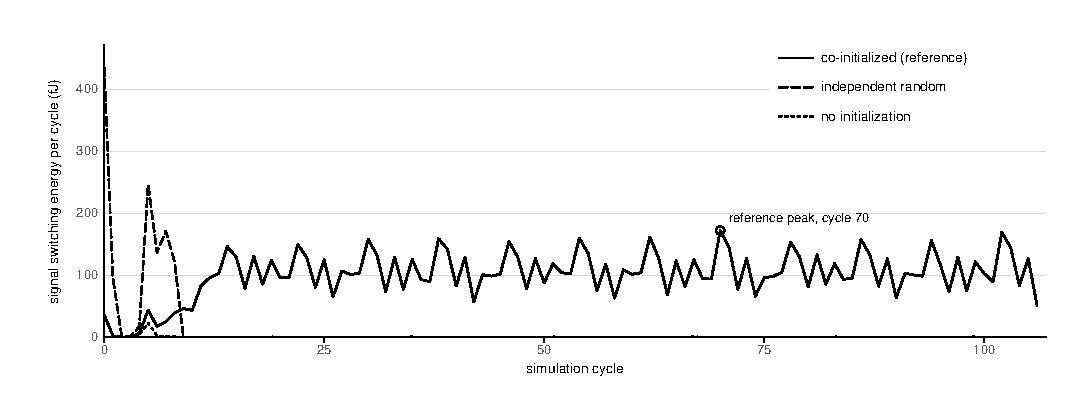
\includegraphics[width=\textwidth]{figures/fig_profile.pdf}
\caption{Per-cycle signal switching energy. The randomized netlist concentrates its
activity in a short burst before halting; the uninitialized netlist is nearly
silent because nets held at \X{} never make a countable transition.}
\label{fig:profile}
\end{figure*}

An uninitialized netlist looks almost idle: nets parked at \X{} never make a
countable transition, so a busy design under-reports activity by 98.9\%
(Table~\ref{tab:power}, Fig.~\ref{fig:activity}). The randomized run errs in a
more dangerous way. It under-reports signal power by 88.6\% and simultaneously
over-reports peak power by 14.0\%, placing the peak at cycle 0 rather than 70
(Fig.~\ref{fig:profile}). Peak magnitude and timing inform power-delivery design,
and both are wrong while the run looks clean.

\subsection{Power-up-state sensitivity}

\begin{figure}[!t]
\centering
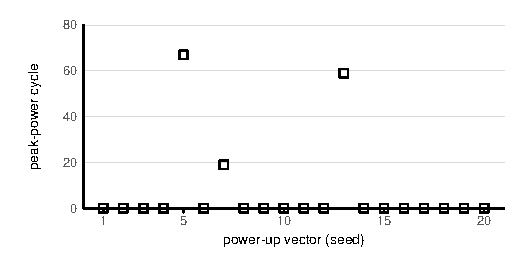
\includegraphics[width=\columnwidth]{figures/fig_sweep_peakcycle.pdf}
\caption{Peak-power cycle for 20 legal power-up vectors, each certified.}
\label{fig:sweeppk}
\end{figure}

\begin{figure}[!t]
\centering
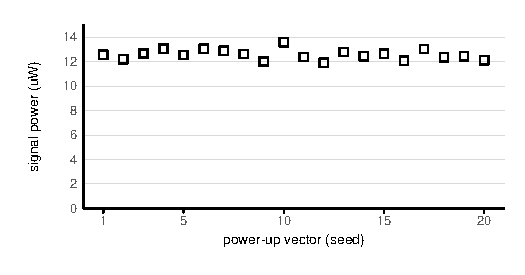
\includegraphics[width=\columnwidth]{figures/fig_sweep_power.pdf}
\caption{Signal power for the same 20 vectors.}
\label{fig:sweeppw}
\end{figure}

Fixing r5 to 0 and randomizing the remaining state gives 20 legal power-up states,
all of which certify and run the full 107 cycles. Across them, transitions range
from 82{,}554 to 93{,}732 (mean 86{,}911, standard deviation 2{,}943), signal power
spans 13.3\% of its mean of 12.57\,\textmu W, total power 0.9\%, and peak power
6.0\% (189.2 to 200.7\,\textmu W). The peak-power cycle takes four different
values, $\{0, 19, 59, 67\}$ (Figs.~\ref{fig:sweeppk} and~\ref{fig:sweeppw}). A
single power number from one arbitrary initialization would conceal all of this.

\subsection{Checkpoint transplant}
RTL state captured at cycle 30 was applied to the netlist, which then ran from
cycle 31 with reset held inactive. Over cycles 31 to 107 the gate-level run matched
RTL in all 77 cycles on every one of the 680 elements. The transplanted run's
median time was 138.9\,ms against 146.5\,ms for the full run, with overlapping
inter-quartile ranges; at this workload length there is no measurable saving, and
this experiment establishes correctness of the transplant rather than a speed-up.

\subsection{Two-state versus four-state comparison}
\label{sec:twostate}

\begin{table}[!t]
\caption{What a two-state comparison sees}
\label{tab:twostate}
\centering\footnotesize
\begin{tabular}{lrr}
\toprule
 & No init & Indep.\ random \\
\midrule
Divergent cycles (four-state)         & 106    & 5 \\
\quad missed entirely by two-state    & 0      & 0 \\
Divergent bit-cycles                  & 56{,}609 & 2{,}706 \\
\quad invisible to two-state          & 46{,}459 & 1{,}339 \\
\quad fraction invisible              & 82.1\% & 49.5\% \\
First detection, both comparisons     & cyc 2  & cyc 1 \\
\bottomrule
\end{tabular}
\end{table}

\begin{figure}[!t]
\centering
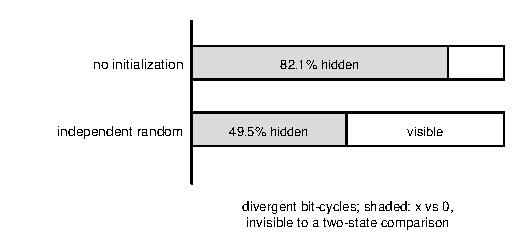
\includegraphics[width=\columnwidth]{figures/fig_twostate.pdf}
\caption{Share of divergent bit-cycles that a two-state comparison cannot see.}
\label{fig:twostate}
\end{figure}

Replaying the recorded state through a two-state comparison, which compares whole
reduced vectors so hash collisions play no part, shows its limits
(Table~\ref{tab:twostate}, Fig.~\ref{fig:twostate}). In both arms it flagged every
divergent cycle at the correct first cycle, because each such cycle contained at
least one bit it could see. But it could not see 82.1\% of the divergent bits in
arm B and 49.5\% in arm C, it cannot classify any divergence as X-origin or
RTL-unknown, and a divergence confined to bits whose reference value is 0 would
pass unnoticed. Detection happening to coincide here is a property of this
workload, not a guarantee.

\subsection{Cost of the method}

\begin{table}[!t]
\caption{Timing, median of 21 runs [inter-quartile range], ms}
\label{tab:time}
\centering\footnotesize
\begin{tabular}{lr}
\toprule
Configuration & Time \\
\midrule
RTL, 107 cycles                         & 12.8 [12.4--14.9] \\
GLS co-initialized, 107 cycles          & 154.6 [132.3--168.9] \\
\quad with per-cycle state dump         & 156.3 [130.4--199.6] \\
GLS without deposit, 1 cycle            & 99.8 [88.3--111.3] \\
GLS with deposit, 1 cycle               & 99.3 [89.9--115.9] \\
Offline four-state compare, 680 flops   & 46.0 [44.2--52.3] \\
Build correspondence map                & 62.9 [61.7--74.5] \\
\bottomrule
\end{tabular}
\end{table}

Every configuration was capped at the same cycle count and interleaved over 21
repetitions (Table~\ref{tab:time}). The deposit changed the one-cycle run by
$-0.5$\,ms and the per-cycle state dump changed the 107-cycle run by $+1.7$\,ms;
both differences are far smaller than the spread between repetitions, so the
method's run-time cost is not measurable at this design size. Building the map and
comparing the state are one-off costs of tens of milliseconds. Gate-level
simulation was about $12\times$ slower than RTL. Each run is a separate process of
well under a second, so start-up cost dominates every figure; these measurements do
not predict per-cycle cost on long workloads or production designs.

\subsection{Cross-simulator confirmation}

\begin{table}[!t]
\caption{core\_small testcase, identical on Icarus 13.0, VCS X-2025.06-SP1 and
QuestaSim 2025.2}
\label{tab:xsim}
\centering\footnotesize
\begin{tabular}{lrrrl}
\toprule
Arm & Arch. & State & Gate & Halts \\
    & div.  & div.  & \X   & RTL / gate \\
\midrule
No init           & 59 & 1{,}449 & 1{,}449 & 12 / never \\
Gate randomized   & 12 & 500     & 0       & 12 / 5 \\
Co-init, 2 seeds  & 0  & 0       & 0       & 5 / 5 \\
Constrained, 3    & 0  & 0       & 0       & 12 / 12 \\
\bottomrule
\end{tabular}
\end{table}

The core\_small testcase runs all arms in one simulation and prints 23 result lines.
Icarus Verilog, Synopsys VCS and Siemens QuestaSim produced identical lines
(Table~\ref{tab:xsim}). No run was given a register-initialization option, and each
reported the full count of unknown values in the uninitialized arm, so the baseline
was not silently pre-initialized. QuestaSim required explicit access options before
hierarchical deposits would bind. Agreement across three independent
implementations indicates the behaviour follows from the language's four-valued
semantics rather than from any one simulator. The testcase's printed labels use two
classes; its randomized-arm divergence has an unknown RTL value and is an
RTL-unknown divergence in the terms of this article.

\section{Discussion}

\subsection{Why removing unknowns does not validate activity}
An unknown-value check answers whether the gate-level run is \emph{determinate}.
Power analysis needs to know whether it is \emph{the workload}. Independent
initialization produces a determinate run of a different workload, and the
determinate run is the more convincing error: 0.0\% unknown transitions, a plausible
activity profile, and a peak in the wrong place. Only a comparison against the
reference execution distinguishes the two.

\subsection{Scaling}
Nothing in the flow depends on design size except the correspondence map and the
per-cycle comparison. At scale the map should come from a formal equivalence
checker, whose matched points survive retiming. The comparison is one four-state
operation per cycle per chunk; comparing at instruction retirement until a failure
and then re-running per cycle bounds cost further. We have not measured these at
production scale.

\subsection{Timing, clock gating and low power}
With delay annotation, activity includes glitches and sampling must follow
settling. Clock-gating enables belong in the compared state, since a mis-modelled
gate changes a whole domain's activity. Retention state and domain power state
extend the vector and qualify the comparison. None of these were exercised here.

\section{Threats to Validity}
The designs are small models, not production silicon. The cell library and energy
table are synthetic, so power magnitudes are illustrative. No delay annotation was
used. Activity, power and timing come from one open-source simulator; the
three-simulator agreement covers only the equivalence results of the 58-element
testcase. Timing measurements are dominated by process start-up. The workload is a
single program chosen to contain a branch on uninitialized state; other workloads
may diverge differently or not at all. The two-state analysis replays recorded
state rather than implementing a two-state comparator inside the simulator.

\section{Conclusion}
Removing unknown values from a gate-level simulation does not make its switching
activity valid. On a 680-element processor, the common mitigation left no unknown
values and reproduced the reference execution in none of 20 seeds, while signal power
was off by 88.6\% and peak-power timing was wrong. Starting both models from one
shared power-up state and admitting activity only for cycles where their full state
agrees reproduced the execution in every seed, exposed a latent dependence on
uninitialized state, and made the sensitivity of peak-power timing to power-up
state measurable. At the scale studied its run-time cost was below timing noise.

\section*{Artifact Availability}
The harness --- RTL, cell library, synthesis scripts, correspondence-map builder,
vector generator, divergence and power tools, the two-file testcase, the
commercial-simulator logs, and the scripts that generate this article's figures ---
is public. \texttt{RUN\_ALL.sh} reproduces every table and figure using only Yosys,
Icarus Verilog and Python.

\begin{thebibliography}{10}
\bibitem{ieee1364} \emph{IEEE Standard for Verilog Hardware Description Language},
IEEE Std 1364-2005.
\bibitem{ieee1800} \emph{IEEE Standard for SystemVerilog---Unified Hardware Design,
Specification, and Verification Language}, IEEE Std 1800-2023.
\bibitem{p8000950} ``Random initialization of latches in an integrated circuit design
for simulation,'' U.S. Patent 8{,}000{,}950, 2011.
\bibitem{p9965575} ``Methods and systems for correcting X-pessimism in gate-level
simulation or emulation,'' U.S. Patent 9{,}965{,}575, 2018.
\bibitem{p10726180} ``Systems and methods for fixing X-pessimism from uninitialized
latches in gate-level simulation,'' U.S. Patent 10{,}726{,}180.
\bibitem{p9058452} ``Systems and methods for tracing and fixing unknowns in gate-level
simulation,'' U.S. Patent 9{,}058{,}452.
\bibitem{p10540462} ``Method and apparatus for speeding up gate-level simulation,''
U.S. Patent 10{,}540{,}462, 2020.
\bibitem{p6598209} ``RTL power analysis using gate-level cell power models,''
U.S. Patent 6{,}598{,}209.
\bibitem{yosys} C.~Wolf, ``Yosys Open SYnthesis Suite.'' [Online]. Available:
\url{https://yosyshq.net/yosys/}
\bibitem{icarus} S.~Williams, ``Icarus Verilog.'' [Online]. Available:
\url{https://steveicarus.github.io/iverilog/}
\end{thebibliography}

\end{document}
